\chapter{Results}

\section{Different backbones}
We changed the batch-size to 2 (to be able to fit 5x6 backbone into the GPU memory) and trained the model with different bacbones for 50 epochs each. Results for all runs are in the table \ref{tab:yolov5_backbones}.

\begin{table}
    \begin{tabular}{c|c|c|c|c|c}
        Backbone & $AP@.5$ & $AP$  & Parameters[M] & Flops[G] & Time[h] \\ \hline
        5s6      & 0.593   & 0.231 & 12            & 21       & 2.1     \\ \hline
        5m6      & 0.621   & 0.242 & 35            & 63       & 3.5     \\ \hline
        5l6      & 0.611   & 0.241 & 76            & 141      & 5.2     \\ \hline
        5x6      & 0.601   & 0.238 & 140           & 267      & 8.5     \\
    \end{tabular}
    \caption{Results of the YOLOv5 architecture with different backbones}
    \label{tab:yolov5_backbones}
\end{table}

\section{Different image size}
Once again we kept the same setting and this time changed only the size to which images are resized. The relation between input image size and $AP@.5$ can be observed in the figure

\begin{figure}
    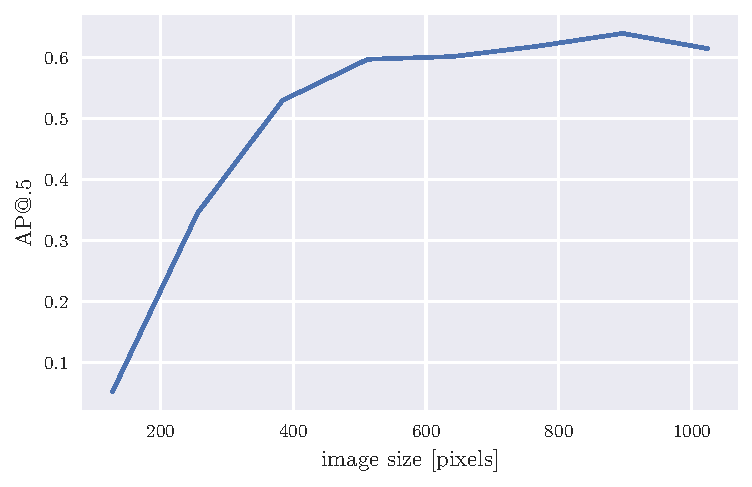
\includegraphics[width=\linewidth]{images/img_size_dependency.pdf}
    \caption{Dependency of $AP@.5$ on the input image size}
\end{figure}
